\documentclass[12pt]{article}
\usepackage[english]{babel}
\usepackage[utf8x]{inputenc}
\usepackage{amsmath}
\usepackage{graphicx}
\usepackage[colorinlistoftodos]{todonotes}
\usepackage{xcolor}
\usepackage{sectsty}
\usepackage{pdfpages}
\usepackage[hidelinks]{hyperref}
\usepackage[top = 100pt, bottom = 100pt, left = 45pt, right = 45pt]{geometry}

\definecolor{netpurple1}{rgb}{0.41, 0.21, 0.61}
\definecolor{netpurple}{rgb}{0.59, 0.47, 0.71}

\begin{document}
\begin{titlepage}

\newcommand{\HRule}{\rule{\linewidth}{0.5mm}} % Defines a new command for the horizontal lines, change thickness here

\center % Center everything on the page

\textsc{\LARGE The Royal Institute of Technology}\\[1.5cm] % Name of your university/college
\textsc{\Large Finance and Control in Industrial Organizations}\\[0.5cm] 
\textsc{\large Control Project}\\[0.5cm] 

\HRule \\[0.4cm]
{ \huge \bfseries Perspectives on Netlight Strategy}\\[0.4cm] % Title of your document
\HRule \\[1.5cm]

\begin{minipage}{0.4\textwidth}
\begin{flushleft} \large
\emph{Authors:}\\
Peter \textsc{Finnman} \\% Your name
Marcus \textsc{Larsson} \\

Mijael \textsc{Rodriguez}
\end{flushleft}
\end{minipage}
~
\begin{minipage}{0.4\textwidth}
\begin{flushright} \large
Simon \textsc{Westerlind} \\
Nick \textsc{Nyman} 
% Supervisor's Name
\end{flushright}
\end{minipage}\\[2cm]

{\large \today}\\[2cm] % Date, change the \today to a set date if you want to be precise

%----------------------------------------------------------------------------------------
%	LOGO SECTION
%----------------------------------------------------------------------------------------
\begin{minipage}{0.3\textwidth}
\begin{flushleft}

\includegraphics[scale=0.1]{kth}\\[1cm] 
\end{flushleft}
\end{minipage}
~
\begin{minipage}{0.3\textwidth}
\begin{flushright}

\includegraphics[scale=0.1]{netlight}
\end{flushright}
\end{minipage}

 
%----------------------------------------------------------------------------------------

\vfill % Fill the rest of the page with whitespace

\end{titlepage}

\sectionfont{\color{netpurple1}}
\subsectionfont{\color{netpurple}}
\begin{abstract}
Your abstract.
\end{abstract}
 \newpage
 
\tableofcontents
\newpage

\section*{Introduction}
\addcontentsline{toc}{section}{Introduction}
One of the most fundamental challenges of any company is one that often requires more attention than it receives. It is difficult to grasp, yet it is central to both the processes and the direction of the company. The corporate strategy provides the  foundation  of the business that ties into every action. \\
\newline\noindent
Netlight Consulting provides its clients with tailored IT and management solutions with focus on innovation and business sense. They employ approximately 700 employees and have offices i 8 cities, including Stockholm, Paris, London and Munich (Netlight LinkedIn, 2016). We have delved into their corporate culture and assessed their strategy with the objective of finding improvements from the perspective of strategy maps and balanced scorecards (Kaplan and Norton, 2004). As industrial management students from a computer science background, conducting a study of this nature yields valuable insight into key success factors of Netlight. Furthermore, it is a tremendous opportunity for us to partake in shaping our future workplace. \\
\newline\noindent
The purpose of this study can be divided in two perspectives. The study allows for practical application of theory introduced in the industrial management program, further expanding our understanding of the interaction between corporate strategy and culture. Additionally, there is great appeal for Netlight to get an outside perspective of their company.

\section*{Analysis of Netlight}
\addcontentsline{toc}{section}{Analysis of Netlight}
An essential part of corporate strategy is the company's mission, vision and values (Kaplan and Norton, 2004). These establish clear guidelines for both employees and clients on the company's purpose, where the company is headed and the embodied values of the company. 
\subsection*{Values}
\addcontentsline{toc}{subsection}{Values}
Netlight has three core values that are at the heart of the company. Their values are \textbf{Competence}, \textbf{Creativity} and \textbf{Business Sense} (Netlight LinkedIn, 2016) which are most of all reflected in the employees that they hire. \\
\newline
Competence is not only reflected in Netlight's recruitment of potential candidates. Perhaps more importantly, it is reflected in their internal processes that ensure that competence grows within the firm. Netlight believes in competence in the form of collective knowledge. Their EDGE program is designed to bring employees together and create an environment where they feel encouraged to share their experience with one another (Netlight LinkedIn, 2016; Interview With Employee at Netlight's Internal Business Development Unit, 2016). Additionally, the corporate culture at Netlight stimulates getting input from employees possessing relevant expertise that are not directly connected to the project. Lastly, all employees at Netlight are equipped with a mentor to coach them in their career. In addition to semi-annual feedback sessions, the mentorship gives employees access to faster feedback which has tremendous impact on individual competence (Interview With Employee at Netlight's Business Development Unit, 2016).\\
\newline
Most companies strive for creativity to varying extents. Netlight believes in individuals but not in individualists (Netlight, 2016). Creativity starts at the individual level and is enhanced at an organizational level to deliver innovative solutions to customers. Furthermore, Netlight realizes one of the key factors to creativity is an open-minded, diverse work force. Their Vostok initiative attempts to attract women into the IT-industry by arranging meet-ups, code pubs and by talking at universities. This gives Netlight the advantage by assuming the role of a familiar face for newly graduated women. \\
\newline
The business sense is essential to the surrounding components of problem solving (Interview With Employee at Netlight's Talent Search, 2016). They don't strive to find the best programmers. Instead, they recruit individuals with a healthy blend of technical competence and business sense that create a good atmosphere when working with customers (Interview With Employee at Netlight's Internal Business Development Unit, 2016). This can be identified as one of the key factors to Netlight's success.
\subsection*{Misson and Vision}
\addcontentsline{toc}{subsection}{Mission and Vision}
Netlight is renowned for their talented workforce and their inclusive and knowledge-based corporate culture. They place a lot of trust in their employees and value a highly autonomous work style. This does not undermine the fact that collaboration is valued as well. This is reflected in the fact that they do not have a clear mission or vision statement. However, the purpose of these statements is to permeate the organization and its employees.\newline

\textit{"As genuine consultants we offer independent solutions, tangible results and sustainable value to our clients through a combination of competence, creativity and business sense."}
\subsection*{Strategy}
\addcontentsline{toc}{subsection}{Strategy}
As a consulting firm, Netlight's strategy type is customer solutions. They rely on returning customers and provide their clients with long-term profitability (Kaplan and Norton, 2004). However, by considering their consultants as products, they fulfill a majority of the criteria of product leadership as well. By incorporating business sense and valuing personality, Netlight can venture into unexplored market segments where technical competence by itself is not adequate. \\
\newline
We mentioned earlier that one of Netlight's core values is competence. This is somewhat misleading since it implies that the competence is tied to individuals. However, by virtue of knowledge sharing within the organization, Netlight brings the entirety of the firm's competence to each customer. Herein lies the corporate strategy. They invest in the acquiring talented individuals in combination with an open and inclusive corporate culture. This translates to good business relations and solutions where a multitude of perspectives are explored.

\section*{Strategy Map}
\addcontentsline{toc}{section}{Strategy Maps}
The strategy map is a simple approach to get a holistic view of the organization. It incorporates four different perspectives and links them together through cause and effect.

\subsection*{Financial Perspective}
\addcontentsline{toc}{subsection}{Financial Perspective}
At the top of the financial perspective is the \textbf{shareholder value}. In 
order to increase the value that Netlight delivers to their shareholders, the company can either \textbf{increase revenue} or \textbf{decrease costs}. Increasing revenue can be accomplished through \textbf{expanding} into new market segments or geographical locations. Alternatively, Netlight can strive to exploit current market segments to a greater extent. Despite not creating value instantaneously, customer retention is essential as it facilitates creating shareholder value in the future.

\subsection*{Customer Perspective}
\addcontentsline{toc}{subsection}{Customer Perspective}
Customer retention is achieved through \textit{genuine consulting} which boils down to maintaining healthy relations with customers. Netlight achieves this by virtue of their three core values: \textbf{competence}, \textbf{creativity} and \textbf{business sense} which is reflected in their recruitment process. These values translate to \textbf{independent solutions} and \textbf{tangible results} of \textbf{significant value} for their customers. Thus, it is imperative to maintain these values when chasing strategic objectives. Thought has to be devoted to both \textit{internal processes} and how the organization \textit{learns and grows}.

\subsection*{Internal Process Perspective}
\addcontentsline{toc}{subsection}{Internal Process Perspective}
We propose alignment with the following objectives within the internal process perspective.
\begin{itemize}
\item \textbf{Streamline administration} - Remove unnecessary administrative tasks (for example HR's invoice tasks) so that employees can focus on their real objectives.
\item \textbf{Improve utilization of consultant's in-house time} - Having tools that make it easy to find consultants between jobs, with relevant expertise, to assist in in-house projects. 
\item \textbf{Education, knowledge sharing and individual improvement} - In order to guarantee cutting edge solutions, Netlight needs to possess cutting edge knowledge. One of the key tools within the company to ensure that knowledge flows between employees is EDGE. EDGE is designed to capture what is important to a client, independent of the technological solutions and deliver it to employees in an inspirational manner. The aim is for the knowledge sharing to become a natural part of the company. The knowledge sharing at Netlight could be improved by two simple measures.
\begin{itemize}
\enlargethispage{\baselineskip}
\item Once a year Netlight hosts an EDGE conference to spread awareness of what is valuable. By hosting some smaller events more frequently Netlight can expect higher morale and more formal networking opportunities.
\item Most of the internal networking is currently ad-hoc based presenting problems in a growing organization. We propose developing platforms facilitating networking between employees. This provides the company with means to minimize growing pains as staff reaches critical mass.
\end{itemize}
\item \textbf{Creating and maintaining customer relations} - Improvements can be made on processes to allow for consultants to focus more on the customer. Netlight's culture embraces chaos. However, by tactically incorporating structure into procedures that are repeated between customers, the aforementioned improvements can be made.
\end{itemize}

\subsection*{Learning \& Growth Perspective}
\addcontentsline{toc}{subsection}{Learning \& Growth Perspective}
\textbf{Human capital} is the importance of recruiting  and maintaining the right individuals for the firm. This encapsulates reflection regarding which individuals to target in the recruitment process.
\begin{itemize}
\item \textbf{Personal networks} - Since Netlight revolves around employee networking, HR should focus on identifying individuals that can communicate their expertise in an understandable manner. Additionally, targeting people with large networks outside of the company provides valuable perspectives as well as a larger talent pool for potential recruitment.
\item \textbf{Self-leadership} - In a consulting firm autonomy is essential. This requires employees that are self-governing and able to promote their ideas. 
\item \textbf{Diversity} - From a recruitment standpoint it is important to show that the company values diversity. By employing and maintaining a diverse workforce the company gains access to new markets segments as well as new ideas.
\end{itemize}
\noindent
\textbf{Information capital} involves efficient handling of information internally, including knowledge bases, business systems and communication platforms.
\begin{itemize}
\item \textbf{Accessible knowledge base} - It should be straight forward to contact other employees with relevant expertise to the project. 
\item \textbf{Easy to handle business systems} - Assist in administrative tasks through intuitive internal business systems.
\item \textbf{Customer Database} - In order for the organization to achieve organizational alignment in regards to a product range, a control system of current customers needs to be implemented.
\end{itemize}

\noindent
\textbf{Organizational capital} entails the routines and culture that ensure that the firm can deliver quality services to its customers.

\begin{itemize}
\item \textbf{Open minded culture} - Engage employees in diversity. Focus on the importance of keeping to company values when meeting clients while still being open. Another side to the same coin is when to disagree. McKinsey \& Company believes in the \textit{obligation to dissent} which helps exhaust all ideas in discussions. The obligation of dissent requires all employees to speak up when they disagree or if presented solutions go against corporate values (McKinsey, 2016). 
\item \textbf{No managers} - In order for employees to be productive they need to feel personal accountability for the product they are developing (Interview With Employee at Netlight's Talent Search, 2016; Thompson, 2004). Therefore, Netlight utilizes a flat hierarchy where managers are replaced with coaches, called \textit{solution managers}.
\end{itemize}
\enlargethispage{2\baselineskip}
\begin{figure}[h!tp]
\hspace*{-20pt}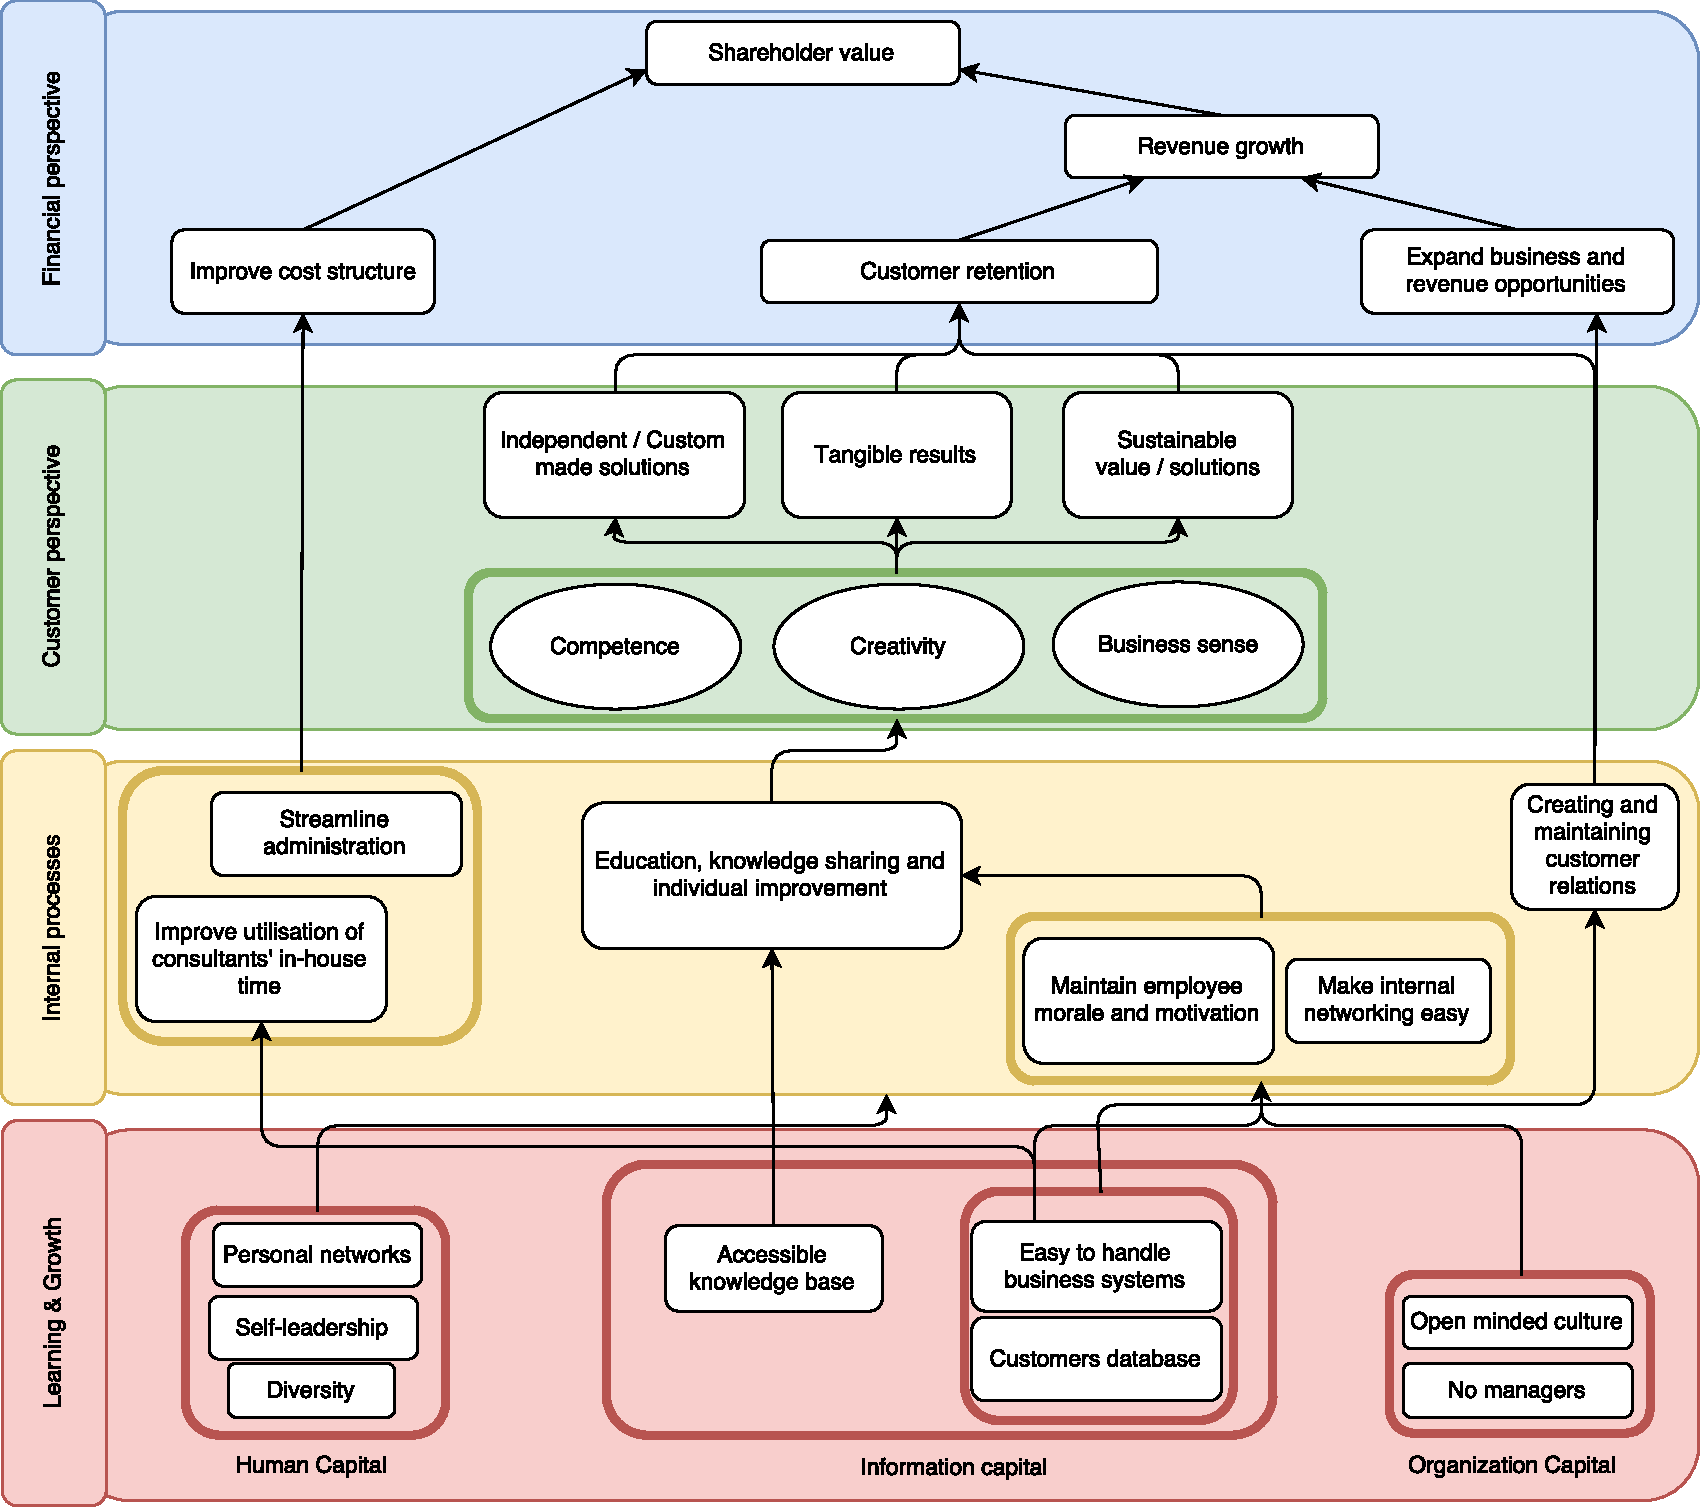
\includegraphics[scale=0.7]{StrategyMap}
\caption{Strategy Map of Netlight Consulting}
\end{figure}

\newpage
\section*{Strategic Themes}
\addcontentsline{toc}{section}{Strategic Themes}
In this section we evaluate two different strategic themes in the strategy map (Kaplan and Norton, 2004). A strategic theme can be seen as a flow of cause and effect events that penetrate all four perspectives that were introduced in the previous section. Looking at the lowest level of the strategy map, namely the learning \& growth perspective, we have listed three strategic objectives.

\subsection*{Increase Efficiency of Internal Operations}
\addcontentsline{toc}{subsection}{Increase Efficiency of Internal Operations}


\subsection*{Customer Value}
\addcontentsline{toc}{subsection}{Customer Value}
\hspace*{5pt}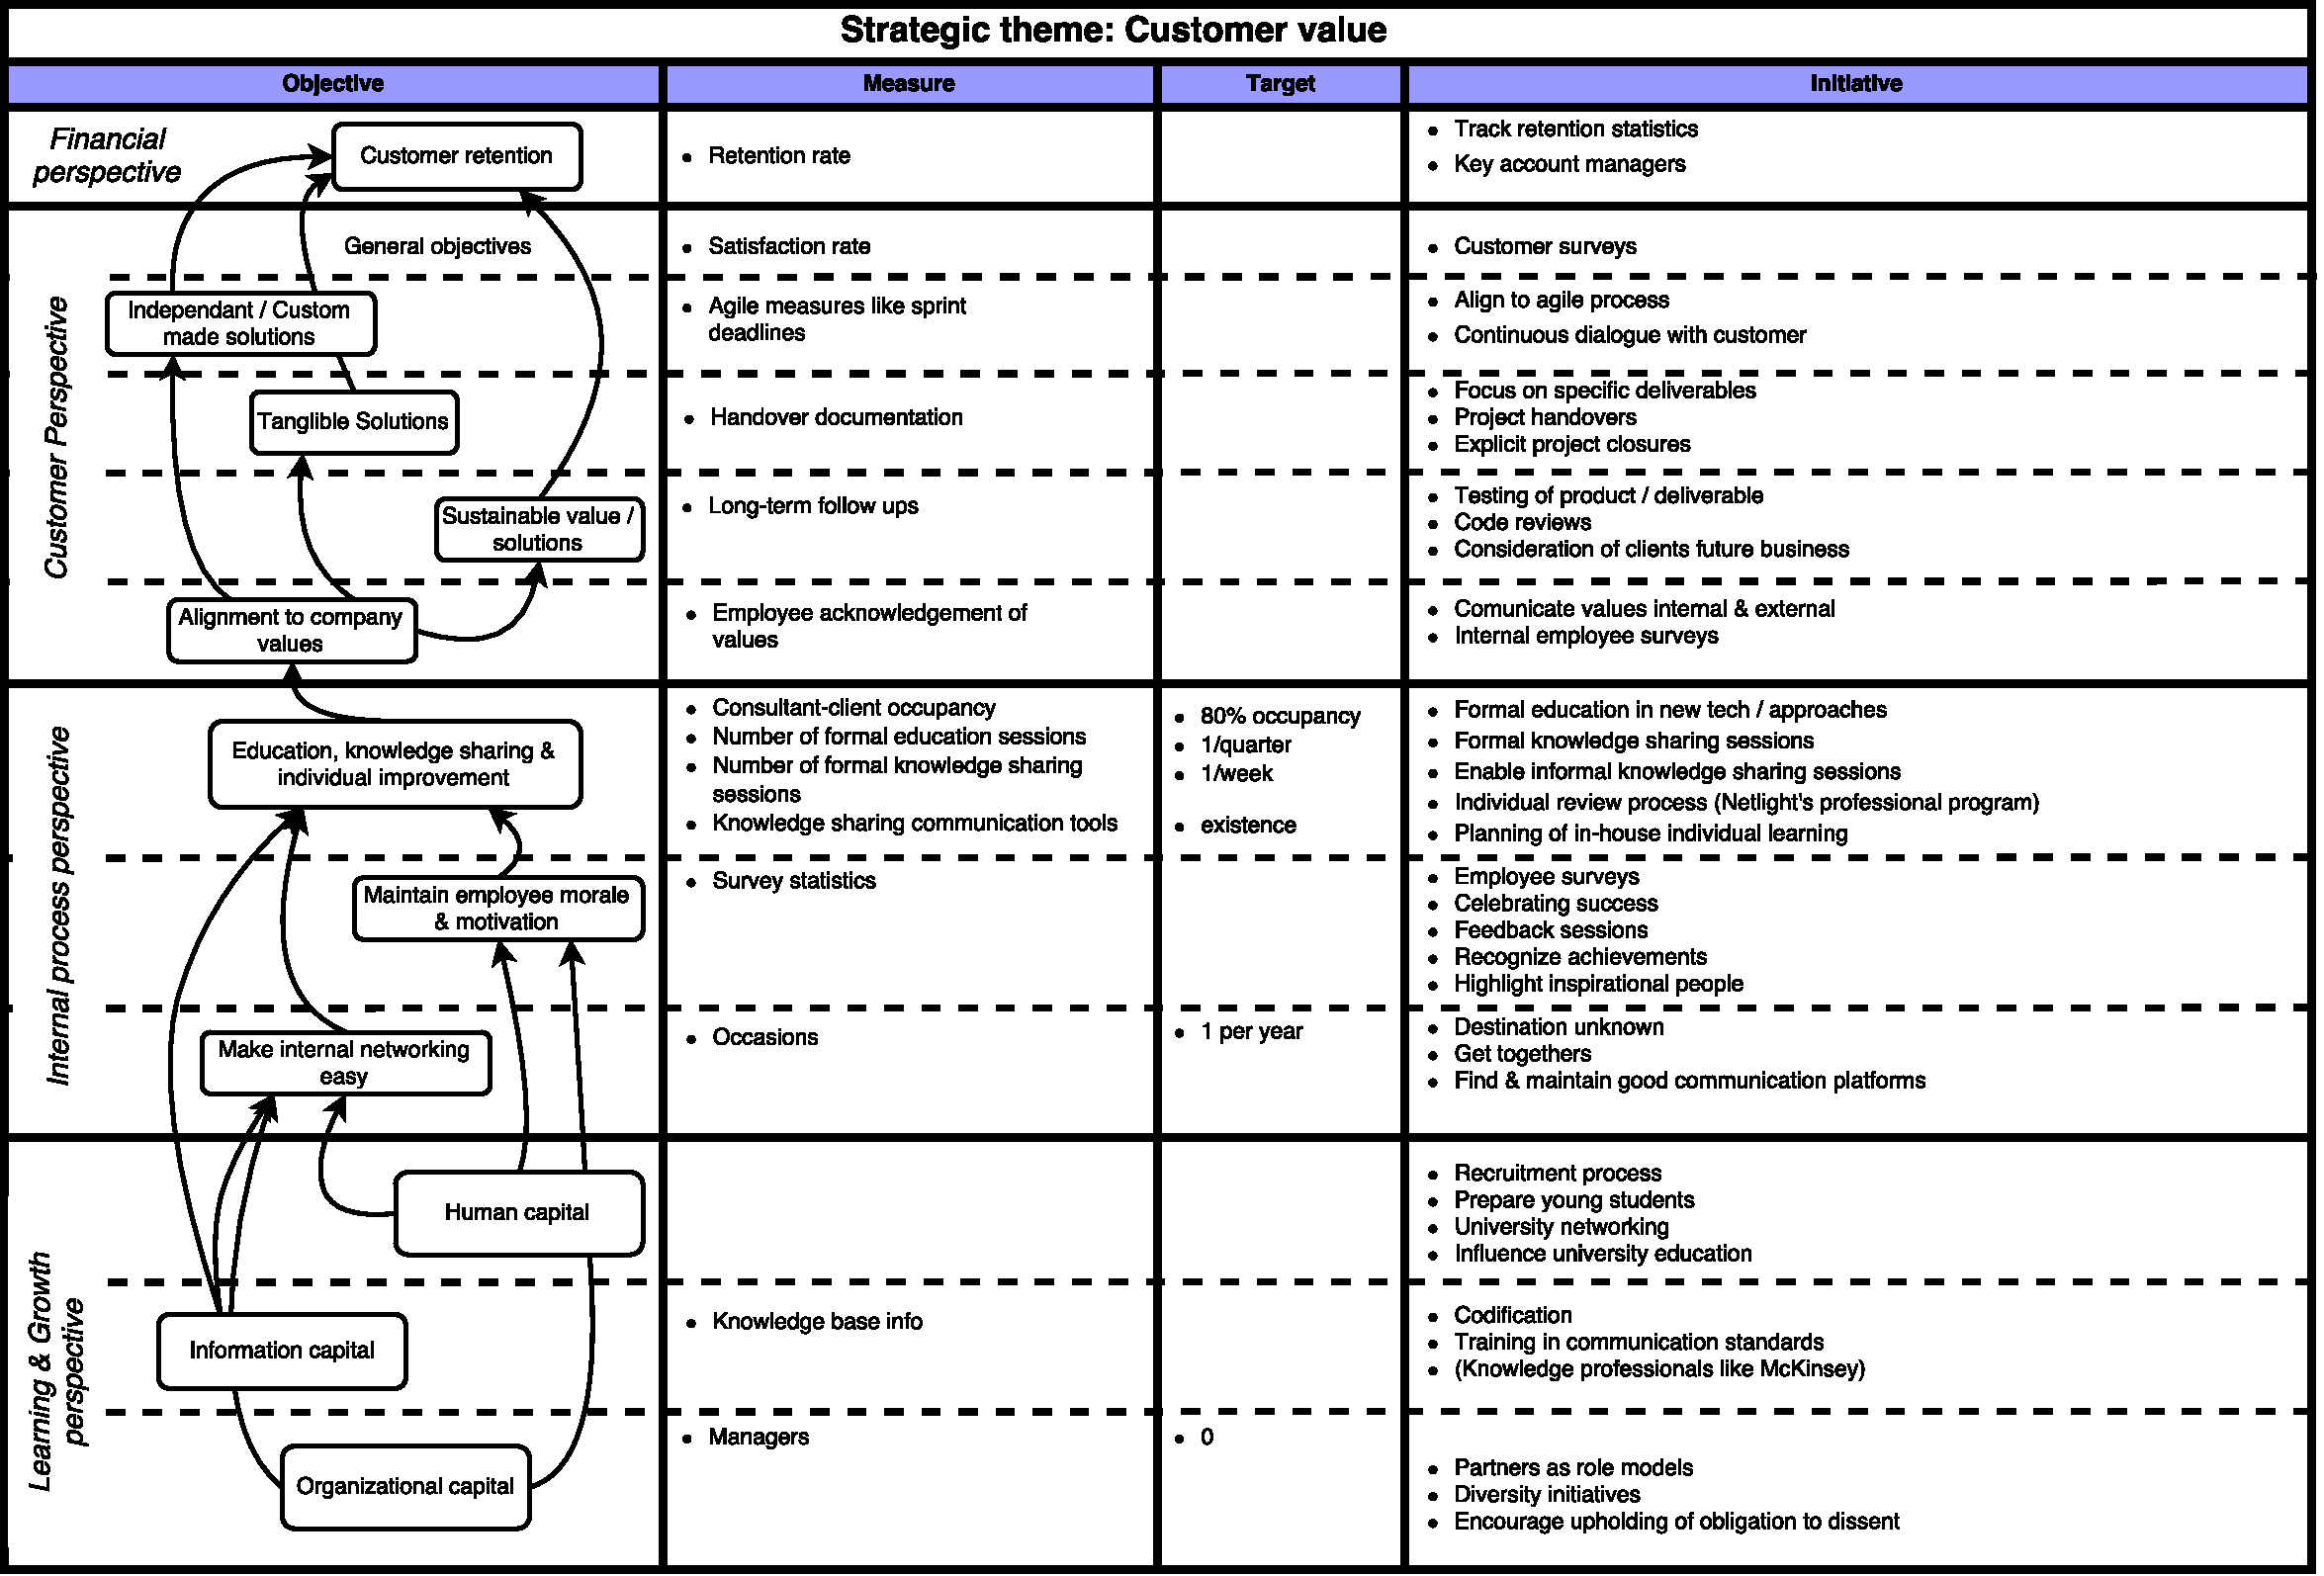
\includepdf[landscape=true]{BalanceScorecard}

\newpage
\section*{Discussion}
\addcontentsline{toc}{section}{Discussion}

\section*{Conclusion}
\addcontentsline{toc}{section}{Conclusion}

\newpage

\makeatletter
\renewcommand\@biblabel[1]{}
\makeatother
\begin{thebibliography}{9}

\bibitem{Kaplan} Kaplan, Robert and Norton, David. (2004). \textit{Strategy Maps}. Boston: Harvard Business School Press. Print.

\bibitem{LinkedIn} Netlight LinkedIn, (2016). [online] Available at: \url{https://www.linkedin.com/company/netlight-consulting/careers?trk=careers_promo_module_desciption} [Accessed 1 Oct. 2016].

\bibitem{Netlight} Netlight, (2016). [online] Available at: \url{https://www.netlight.com/about-us/} [Accessed 2 Oct. 2016].

\bibitem{Interview 1} Interview With Employee at Netlight's Internal Business Development Unit. (2016). Netlight Offices, Birger Jarlsgatan 7. in person.

\bibitem{Interview 2} Interview With Employee at Netlight's Talent Search. (2016). Netlight Offices, Birger Jarlsgatan 7. in person.

\bibitem{Thompson} Thompson, Leigh. (2014). \textit{Making the Team - A Guide for Managers}. 5th Ed. Upper Saddle River, NJ: Prentice Hall. Print.

\bibitem{McKinsey} McKinsey. (2016). Our mission and values. [online] Available at: \url{http://www.mckinsey.com/about-us/what-we-do/our-mission-and-values}. [Accessed 3 October 2016].

\end{thebibliography}
\end{document}